\section{Jeu de données données USPS}

Cette partie s'intéresse à la prise en main et au pré-traitement des données.

\subsection{Construction du jeu de données}
Le jeu de données se trouve dans le fichier \texttt{usps\_all.mat} et est représenté par un tenseur \texttt{data} d'ordre $3$. Les dimensions du tenseur sont $256\times 1100 \times 10$.

\begin{lstlisting}
load("usps_all.mat"); % charger 'data'
data = double(data);
\end{lstlisting}

Chaque colonne \texttt{data(:,j,k)} est la vectorisation d'une image , pour laquelle l'indice \texttt{k} correspond à une classe (de 0 à 9) et l'indice \texttt{j} correspond à un échantillon (ici, un exemple du chiffre). Ainsi, la première dimension correspond aux pixels, la deuxième aux chiffres, et la troisième aux classes, comme montré dans la figure ci-dessous. L'ordre des classes est '1', '2', '3', $\ldots$, '0'.

\begin{center}
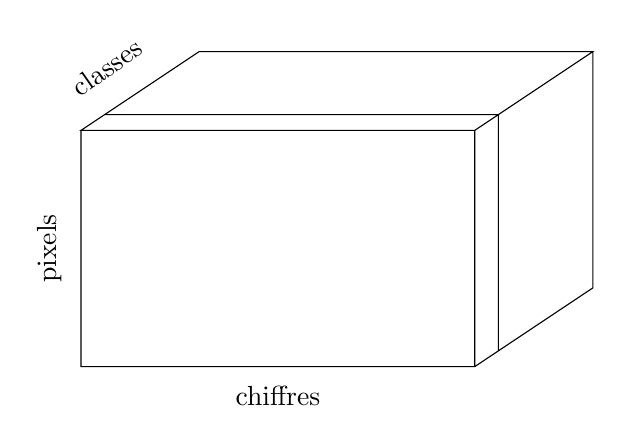
\begin{tikzpicture}

\begin{scope}
	\coordinate (s0) at (0,0);
	\coordinate (s1) at ([xshift=5cm]s0);
	\coordinate (s2) at ([yshift=-3cm]s1);
	\coordinate (s3) at ([yshift=-3cm]s0);
	\coordinate (s4) at ([xshift=1.5cm,yshift=1cm)]s0);
	\coordinate (s5) at ([xshift=5cm]s4);
	\coordinate (s6) at ([yshift=-3cm]s5);
	%
	\coordinate (s7) at ([xshift=0.3cm,yshift=0.2cm)]s0);
	\coordinate (s8) at ([xshift=5cm]s7);
	\coordinate (s9) at ([yshift=-3cm)]s8);
\end{scope}

\draw 
	(s0) -- (s1) -- (s2) -- node[label=below:chiffres] {} (s3) -- node[label=left:{\rotatebox{90}{pixels}}] {} cycle
	(s0) -- node[label={[xshift=3mm,yshift=3mm]left:{\rotatebox{35}{classes}}}] {} (s4) -- (s5) -- (s1) -- cycle
	(s5) -- (s6) -- (s2)
	(s7) -- (s8) -- (s9);

\end{tikzpicture}
\end{center}


\begin{enumerate}
	\item Afficher quelques exemples des images d'entraînement, dans les classes 7 et 9 par exemple, à l'aide de \texttt{imagesc}.
%\begin{lstlisting}
%colormap(gray);
% Insérer votre code ici
%\end{lstlisting}

	\item En apprentissage automatique, il est d'usage de séparer le jeu de données en deux parties: une partie servant à l'entraînement du modèle, l'autre à sa validation. Diviser le jeu de données en deux tenseurs \texttt{T} et \texttt{V}, en sélectionnant des sous-tenseurs de data selon la deuxième dimension (chiffres). Les indices \texttt{ind\_train} et \texttt{ind\_valid} correspondant aux échantillons à extraire dans chaque sous-tenseurs sont donnés dans le fichier \texttt{usps\_partition.mat}, qui se charge comme avant avec la commande \texttt{load}.
\end{enumerate}

\subsection{Analyse en composantes principales (ACP)}

\begin{enumerate}
\setcounter{enumi}{2}
\item Pour les données d'entraînement \texttt{T}, calculer le dépliement du tenseur \texttt{T} selon le mode 1 (une matrice avec 256 lignes) à l'aide de la commande \texttt{reshape}, et trouver la matrice \texttt{U} des dix premiers vecteurs singuliers gauches du résultat. %(commande \texttt{svd}).

\item Replier chaque vecteur singulier en une matrice  $16 \times 16$ à l'aide de \texttt{reshape} et les afficher avec \texttt{imagesc} dans une même figure.
\end{enumerate}

Nous allons entraîner un classifieur SVM sur deux des 10 classes (les chiffres 7 et 9).

\begin{enumerate}
\setcounter{enumi}{4}
\item Sélectionner dans \texttt{T} les données des deux classes 7 et 9, et convertir ces données labellisées en: 1) une matrice \texttt{Xt(chiffre,pixel)} de $256$ colonnes, et 2) un vecteur \texttt{yt(classe)} de labels.

\item Décomposer de même les données de validation en matrice \texttt{Xv} et vecteur \texttt{yv}.

\item %Les colonnes de la matrice \texttt{U} calculée précédemment engendrent un espace vectoriel de faible dimension (ici 10), qui est une (bonne) approximation de l'image de \texttt{X}. L'ACP consiste à projeter nos données sur cet espace de dimension réduite ($\tilde{X} = XU$). Effectuer cette ACP.
Pour les données d'entraînement, appliquer la réduction de dimension pour passer de l'espace de dimension 256 à l'espace de dimension 10 ($\widetilde{\X} = \X\U$).
\end{enumerate}